% ============================================================
% Submission target: IUCrJ (research letter / short communication)
% Base class: article (compiles anywhere). To submit, the body below
% drops into the IUCr class with \documentclass{iucr} and \journalcode{J}.
% ============================================================
\documentclass[11pt]{article}
\usepackage[utf8]{inputenc}
\usepackage[T1]{fontenc}
\usepackage{amsmath,amssymb}
\usepackage{graphicx}
\usepackage[margin=1in]{geometry}
\usepackage{siunitx}
\usepackage{textcomp}
\usepackage{booktabs}
\usepackage[hidelinks]{hyperref}
\usepackage{authblk}

% --- convenience macros ---
\newcommand{\Ang}{\text{\AA}}
\newcommand{\Gmet}{\mathbf{G}}
\newcommand{\Pop}{\mathbf{P}}
\newcommand{\Uop}{\mathbf{U}}
\newcommand{\Mop}{\mathbf{M}}
\newcommand{\Bbasis}{\mathbf{B}}
\newcommand{\rootinv}{\rho}

\title{\bfseries A load of unit cells: setting-invariant search,
exact reindexing, and lattice trajectories}

\author[1]{[Author One]}
\author[1]{[Author Two]}
\affil[1]{[Affiliation], [City], [Country]}
\date{}

\begin{document}
\maketitle

% ------------------------------------------------------------
\begin{center}
\begin{minipage}{0.92\textwidth}
\small\noindent\textbf{Synopsis.}
A complete root invariant removes orbit enumeration from lattice-similarity
search; retaining the integer map to a canonical obtuse superbase then lifts
any match back to the exact reindexing coset. The construction is demonstrated
on 1361 archival lysozyme cells, a 12\,474-crystal serial XFEL data set, and
continuous deformation trajectories.
\end{minipage}
\end{center}

\begin{abstract}
\noindent
A unit cell is a basis, not a lattice identifier. In the $G^6$ and $S^6$
formalisms, crystallographically equivalent bases occupy an orbit, so a correct
distance requires alternative reduced-cell images, 24 Selling-superbase
permutations, and, near reduction boundaries, transformed paths through
adjacent regions --- robust, but expensive at scale. We instead use the root
form of an obtuse superbase as a complete, continuous lattice invariant
[Kurlin, 2022]: equality of root invariants tests isometry directly, and
proportionality tests similarity, with no orbit search at query time. The basis
information the invariant deliberately discards is recovered by retaining the
integer coordinates of the canonical superbase, so that for matched cells $A$
and $B$ the change of basis is an exact integer matrix
$\Pop = \Uop(A)\,\Uop(B)^{-1}$ with $\Pop^{\mathsf T}\Gmet(A)\Pop = \Gmet(B)$;
symmetry-related solutions form a coset, not a single operator. This
\emph{quotient-then-lift} construction is realised in a dependency-free package
and validated on real data at three scales. All 1361 hen egg-white lysozyme
cells in the PDB --- six space groups, four crystal systems --- collapse onto
one setting-invariant metric in which the dominant tetragonal form resolves
into a continuous 1113-cell dehydration trajectory whose intrinsic (Laplacian)
coordinate recovers cell shrinkage at $|r| = 0.92$. A 12\,474-crystal serial
XFEL data set (\mbox{CXIDB 83}, $\beta$-lactamase, $P6_3$) is parsed from its
CrystFEL stream and its full per-pattern indexed-cell distribution --- hidden
entirely by the single merged deposition --- is exposed; mapping crystal
orientation onto the orientation-blind invariant reveals that the long
\SI{233}{\angstrom} axis is measured about $3\times$ worse when the beam looks
down it, a sampling artifact separable from true lattice spread. On benchmarks
the root invariant indexes 3000 cells in \SI{0.04}{\second} with
\SI{0.02}{\milli\second} median nearest-neighbour queries (a
\SI{6}{\text{-dimensional}} \texttt{scipy} KD-tree on the root vector; the
full PDB, 206\,214 cells, builds in \SI{0.28}{\second} with \SI{0.04}{\milli\second}
median $k{=}10$ queries), and reduces a 200-frame serial reindexing problem from
\SI{23}{\milli\second} to \SI{0.07}{\milli\second} per frame for a cached
two-operator reference coset.

\medskip
\noindent\textbf{Keywords:} unit-cell databases; root invariants; serial
crystallography; reindexing; lattice trajectories; nearest-neighbour search.
\end{abstract}

% ------------------------------------------------------------
\section{Introduction}

Modern diffraction workflows produce unit cells much faster than refined
structures. A structural database holds hundreds of thousands of reported cells;
a serial experiment indexes tens of thousands of snapshots; a thermal, pressure,
or operando experiment yields a densely sampled sequence of slightly different
cells. These are usually treated as three separate software problems. They share
a more basic difficulty: the measured six-tuple
$(a, b, c, \alpha, \beta, \gamma)$ describes a \emph{basis}, whereas the object
to be compared is the \emph{lattice} it generates.

Let $\Bbasis$ be a direct-space basis and $\Gmet = \Bbasis^{\mathsf T}\Bbasis$
its metric tensor. Every unimodular integer matrix $\Mop$ gives another basis of
the same lattice, $\Bbasis' = \Bbasis\Mop$, hence another metric representation
\begin{equation}
\Gmet' = \Mop^{\mathsf T}\,\Gmet\,\Mop .
\end{equation}
A lattice comparison based on one point $\Gmet$ must therefore be invariant over
the entire $\mathrm{GL}(3,\mathbb{Z})$ orbit.

\emph{The origin of the ``six''.} A lattice determined up to rotation is exactly
its metric tensor: two bases give the same rotation class iff their metric
tensors are equal. A metric tensor is a symmetric, positive-definite $3\times3$
matrix, and symmetric $n\times n$ matrices form a linear space of dimension
$n(n+1)/2$, which for $n=3$ is six. The positive-definite ones fill an open
convex cone inside that space. Hence the space of three-dimensional
lattices-up-to-rotation \emph{is} a six-dimensional open convex cone of
positive-definite ternary quadratic forms; the six components are not an
arbitrary packaging of $(a,b,c,\alpha,\beta,\gamma)$ but linear coordinates on
this cone. This is the principled reason a six-dimensional representation exists.
The $G^6$ construction [Andrews \& Bernstein, 1988] takes these coordinates
directly,
\begin{equation}
\mathbf{g} = \bigl(a^2,\; b^2,\; c^2,\; 2bc\cos\alpha,\; 2ac\cos\beta,\;
2ab\cos\gamma\bigr),
\end{equation}
whose decisive property is linearity: the basis change $\Bbasis \to \Bbasis\Mop$
acts on $\mathbf{g}$ by the \emph{linear} congruence $\Gmet \mapsto
\Mop^{\mathsf T}\Gmet\Mop$ of equation~(1), so reduction becomes the geometry of
the cone cut by the discrete group $\mathrm{GL}(3,\mathbb{Z})$ --- polytopes and
faces --- rather than a search in lengths and trigonometric angles. The $S^6$
construction [Andrews \textit{et al.}, 2019] charts the same cone more
symmetrically: it adjoins a fourth superbase vector $v_0 = -(v_1+v_2+v_3)$ and
coordinates by the six pairwise products $s_{ij} = v_i\!\cdot\!v_j$
($0 \le i < j \le 3$). The redundant vector buys symmetry --- the governing group
becomes the 24 permutations $S_4$ of the four superbase vectors, more transparent
than Niggli's case list --- at the cost of a six-of-four redundancy the
comparison must respect.

Reduction makes the orbit finite in practice but does not remove its quotient
geometry. In $G^6$, Niggli reduction selects a fundamental region whose boundary
faces must be identified by reduction transformations; it is exactly on those
faces that an arbitrarily small metric change flips the selected cell (the
reduction-flip ambiguity). In $S^6$, Selling (Delaunay) reduction drives all six
products non-positive --- an obtuse superbase --- which is simpler, but a general
reduced lattice still has 24 equivalent presentations from the $S_4$ relabelling
of superbase vectors, and a correct $S^6$ distance must compare these and examine
boundary-transformed paths when a product approaches zero [Andrews \& Bernstein,
1988, 2014; Andrews \textit{et al.}, 2019; Andrews \& Bernstein, 2023]. This
orbit-and-boundary machinery is not an implementation accident; it is how a
many-to-one basis representation becomes a metric on lattices. The root form
(Section~2) is built from this $S^6$ chart: it takes square roots of the
non-negative conorms $-s_{ij}$ and canonicalises them by a type-dependent
ordering under superbase relabelling, which is
what turns the redundant superbase coordinates into a complete, orbit-free
invariant.

A concrete example is the primitive orthorhombic cell
$(10, 12, 20, 90\degree, 90\degree, 90\degree)$. One Selling presentation is
$[0, 0, 0, -100, -144, -400]$, but relabelling the four superbase vectors
produces 24 equally valid $S^6$ vectors [Andrews \textit{et al.}, 2019], so a
comparison between two single $S^6$ vectors can miss an exact match. Near a
reduction boundary the problem is sharper: an arbitrarily small perturbation can
change which reduced representative is selected. In our boundary-straddling test
the distance between raw reduced $S^6$ representatives changed from 0.08 to 83.7
although the physical perturbation was identical on either side; the
corresponding root-form distance stayed at 0.0010 on both sides. For a single
comparison the additional images are manageable; repeating the orbit work for
every database candidate or every serial frame is the computational problem
addressed here.

The root-form construction changes the order of operations. An obtuse superbase
is four vectors $v_0, \dots, v_3$ summing to zero with non-positive pairwise
scalar products. Its six conorms $p_{ij} = -v_i\!\cdot\!v_j$ are non-negative;
their square roots, ordered by Voronoi type, give a uniquely ordered root
invariant $\rootinv(\Lambda)$. Kurlin (2022) proved that two three-dimensional
lattices are isometric iff their root invariants coincide, and similar iff the
invariants are proportional. Hence
\begin{align}
\rootinv(\Lambda_A) &= \rootinv(\Lambda_B)
   && \text{(isometry)}, \\
\rootinv(\Lambda_A)/\sqrt[3]{V(A)} &= \rootinv(\Lambda_B)/\sqrt[3]{V(B)}
   && \text{(similarity)}.
\end{align}
The root invariant is a \emph{quotient coordinate}: all equivalent bases map to
one continuous point before any search. Approximate matches are ranked with the
Euclidean root-space metric defined in Section~2.1 (equation~\eqref{eq:dist})
[Bright \textit{et al.}, 2021]. Unlike $G^6/S^6$
distance calculations, no orbit or boundary-path enumeration is required per
query.

The invariant cannot, by itself, report a reindexing operator: the basis labels
were intentionally removed. That information is recovered by retaining the
integer transformation accumulated during Selling reduction. Let $\Uop(A)$ and
$\Uop(B)$ hold three independent vectors of matched canonical superbases,
expressed in the original bases of $A$ and $B$. For a compatible superbase
labelling,
\begin{equation}
\label{eq:lift}
\Pop = \Uop(A)\,\Uop(B)^{-1}, \qquad
\Pop^{\mathsf T}\,\Gmet(A)\,\Pop = \Gmet(B).
\end{equation}
Because $\Uop(A)$ and $\Uop(B)$ are unimodular integer matrices, $\Pop$ is an
\emph{exact} integer change of basis; floating-point tolerances enter only when
noisy metrics are verified. A generic root form fixes the superbase
correspondence directly; at degeneracies, the finite superbase permutations
compatible with equal root products are tested. If the lattice has non-trivial
automorphisms the answer is necessarily a coset,
$\mathrm{H}(A)\Pop = \Pop\,\mathrm{H}(B)$, not a unique matrix --- a feature,
since in serial crystallography the residual cosets relative to the crystal Laue
group are exactly the indexing branches that intensities must distinguish.

This quotient-then-lift construction is the common thread of the present work,
and we validate it not on synthetic cells alone but on real data at three scales:
an entire single-protein census from the PDB, a complete serial XFEL indexing
stream, and continuous deformation series. The continuous question --- \emph{how
similar are the lattices?} --- is answered before the discrete question ---
\emph{which basis transformation applies?}

\emph{What is established, and what this paper contributes.} The mathematical
foundation is not new here. The complete, continuous isometry classification of
three-dimensional lattices --- the root invariant, its completeness and
continuity, and the Voronoi-type canonicalisation --- is due to Kurlin (2022),
building on the lattice-representation programme of Andrews \& Bernstein
($G^6$, 1988) and Andrews \textit{et al.} ($S^6$, 2019); Selling and Delaunay
reduction, Le Page metric-symmetry analysis, and the coset structure of
reindexing are all classical. This result settles, in principle, the
lattice-comparison problem that crystallography has approached with
tolerance-gated reductions --- yet it has not been transported into
crystallographic practice or software. The two are, at present, in
non-overlapping publication ecosystems: the completeness result lives in the
lattice-geometry and computational-geometry literature, while the diffraction
pipelines that would use it are built and reported within the crystallographic
$G^6/S^6$/Niggli tradition, and recognising a reduction flip as a
section-versus-invariant problem requires a background (quotient spaces, Delaunay
theory, the topology of the reduced-cell cone) that sits at an unusual
intersection. This paper is the bridge. Its contributions are not new theorems
but (i) the transport of Kurlin's invariant into crystallographic cell comparison
and serial-crystallography reindexing, stated in the field's own terms; (ii) the
synthesis showing that the invariant closes a specific, named, silent failure of
tolerance-gated reindexing by separating a tolerance-free detection step from an
exact, finite operator-recovery step, and that this flip-immunity is the
traversability guarantee a continuous ``lattice manifold'' requires; (iii) a
dependency-free reference implementation; and (iv) a demonstration at data scale
--- a full single-protein PDB census, a complete serial XFEL stream, and
continuous deformation series.

% ------------------------------------------------------------
\section{The root invariant and the reindexing lift}

\subsection{Construction of the root invariant}

We give the construction explicitly, since the whole method rests on it. Start
from a lattice basis $v_1, v_2, v_3$ and form the \emph{superbase} by adjoining
$v_0 = -(v_1 + v_2 + v_3)$, so the four vectors sum to zero. The six
\emph{conorms} are the negated pairwise scalar products
\begin{equation}
p_{ij} = -\,v_i \!\cdot\! v_j, \qquad 0 \le i < j \le 3 .
\end{equation}
A superbase is \emph{obtuse} (equivalently, Selling-reduced) when all six conorms
are non-negative, i.e. every pair of superbase vectors is non-acute. Selling's
theorem guarantees that a finite sequence of reduction steps --- each replacing
the superbase vector pair with the most negative product by a sign-corrected
combination --- reaches such a superbase for any lattice, and the conorms are
then the squared edge lengths of the lattice's Voronoi (Dirichlet) cell. The six
conorms already determine the lattice up to isometry, but not uniquely as
written: relabelling the four superbase vectors permutes the $p_{ij}$ under the
symmetric group $S_4$ (24 elements), and at special metrics several conorms
vanish, placing the lattice on one of Voronoi's characteristic coincidence types
where distinct permutations coincide.

The root form resolves both the redundancy and the boundary behaviour. Define the
six \emph{root products} as the square roots of the conorms,
\begin{equation}
r_{ij} = \sqrt{p_{ij}} \;\ge\; 0 ,
\end{equation}
and collect them into the $2\times3$ \emph{root form}, whose columns hold the
three ``opposite'' pairs $(r_{23}, r_{01})$, $(r_{13}, r_{02})$, $(r_{12}, r_{03})$
--- each a superbase-vector pair and its complement. The root invariant
$\rootinv(\Lambda)$ is the canonical, uniquely ordered representative of this root
form under relabelling [Kurlin, 2022, Def. 5.1]. The ordering rule is
\emph{Voronoi-type dependent}, because the number of vanishing conorms fixes how
much freedom remains: for a generic lattice (type V1, all conorms non-zero) the
full 24 index permutations order all six products into an increasing top row with
tie-broken bottom row; at the more symmetric types the zero pattern leaves fewer
free products (five, four, four, three for V2--V5), ordered by the residual
symmetry of each type --- for example, V2 orders its non-zero products by the
smaller group of the surviving $2\times2$ submatrix, and V3--V5 simply place their
non-zero products in increasing order. In every case the result is a single
canonical tuple, so the invariant is well defined and the comparison never
enumerates the orbit. Taking square
roots is not cosmetic. The conorms scale linearly with an overall lattice
dilation whereas edge lengths scale linearly with the metric \emph{amplitude};
in root ($r_{ij}$) coordinates a uniform scaling of the lattice by $\lambda$
multiplies every component by $\lambda$, so \emph{shape} lives in the direction of
$\rootinv$ and \emph{size} in its magnitude --- which is exactly what makes the
similarity test~(4) a simple proportionality.

Two properties of Kurlin's (2022) invariant are what the method uses.
\emph{Completeness}: for the full root invariant,
$\rootinv(\Lambda_A) = \rootinv(\Lambda_B)$ if and only if
$\Lambda_A$ and $\Lambda_B$ are isometric --- no false coincidences, and a genuine
bijection between lattices-up-to-isometry and root invariants, so in principle
nothing is lost by discarding the basis (our implementation realises this exactly
for the symmetric Voronoi types and, for the generic triclinic type, as the
similarity key discussed below). \emph{Continuity}: $\rootinv$ is Lipschitz-continuous in
the lattice, and in particular stays continuous \emph{across} the Voronoi-type
boundaries where raw Selling or Niggli representatives jump. This is the property
that fails for unprocessed $S^6$ or $G^6$ vectors: in our boundary-straddling
test the raw reduced-representative distance jumped $0.08 \to 83.7$ across a type
boundary while $|\rootinv_A - \rootinv_B|$ stayed at $0.0010$ on both sides.
Because the canonicalisation is a finite ordering rather than a numerical
minimisation over the orbit, computing $\rootinv$ costs one Selling reduction plus
a fixed relabelling --- no per-query orbit search.

\emph{Why the root invariant does not suffer a reduction flip.} It is worth
stating explicitly why continuity holds, because the reduction flip is precisely
the failure it avoids. Reduction --- Niggli or Selling --- \emph{selects} one
cell per lattice, a section of the map from lattices to the
$\mathrm{GL}(3,\mathbb{Z})$ orbit space. That orbit space has a fundamental domain
whose boundary faces are identified in pairs (the same lattice reached by two
integer bases), and a section must choose which face to sit on; near such a face
an arbitrarily small metric change tips the choice to the other basis, whose cell
parameters differ, and the reported cell jumps. The jump is the flip, and it is
unavoidable for \emph{any} scheme that selects a representative, because no
globally continuous section of this quotient exists; in monoclinic it is the
familiar near-degenerate $b$-axis cell-choice instability. The root invariant is
not a section: $\rootinv(\Lambda)$ is constant on the whole orbit and lives on the
quotient itself, where the glued boundary is an ordinary interior point and a
continuous function has no reason to jump. Concretely, the two competing bases at
a flip boundary give root-product tuples that are permutations of one another, and
\emph{at} the boundary a conorm passes through zero so the two crossing products
become equal; canonicalisation by sorting is invariant under that permutation and
varies smoothly through the crossing (the pair $(\min,\max)$ is continuous even as
its two arguments exchange), while the square root is continuous through the
vanishing conorm. The permutation ambiguity that \emph{causes} the Niggli flip is
exactly the ambiguity the sorted canonical form quotients away. This flip-immunity
is unconditional --- it holds for every Voronoi type, including generic triclinic
--- and is independent of the type-dependent injectivity discussed above, which
concerns whether two \emph{different} lattices can collide, not whether one
lattice's representatives are stable.

\emph{The distance between two lattices.} Once each lattice is reduced to its
ordered root invariant the comparison is elementary. We write every invariant as
a length-six vector by padding the vanishing positions of the higher-symmetry
Voronoi types with zeros --- type V$k$ contributes $6,5,4,4,3$ non-zero
components for $k=1,\dots,5$, and the zeros occupy the same ordered slots for
every lattice --- so invariants of \emph{different} crystal systems live in one
common $\mathbb{R}^6$ and are directly comparable. The isometry distance is then
the ordinary Euclidean norm of the difference,
\begin{equation}
\label{eq:dist}
d(\Lambda_A, \Lambda_B) \;=\; \lVert \rootinv(\Lambda_A) - \rootinv(\Lambda_B)
\rVert_2 \;=\; \Bigl(\textstyle\sum_{k=1}^{6}
\bigl(\rootinv_k(\Lambda_A) - \rootinv_k(\Lambda_B)\bigr)^2\Bigr)^{1/2},
\end{equation}
which is a pseudometric on lattices --- symmetric, non-negative, and satisfying
the triangle inequality because it is a Euclidean norm --- carrying physical
length units (\r{A}), since each root product is a square-rooted conorm [Bright
\textit{et al.}, 2021]. It separates isometry classes ($d = 0$ iff isometric)
exactly on the symmetric Voronoi types V2--V5, where the sorted invariant
coincides with Kurlin's complete invariant. For the generic triclinic type V1 our
implementation orders the root products as a sorted multiset and thereby drops
the column pairing of the $2\times3$ root form that the complete invariant
retains; this is collision-free on random triclinic lattices in our tests but is
a similarity key rather than a proven-injective one, which is sufficient for
metric nearest-neighbour ranking, where a candidate is in any case confirmed by
the exact operator test of Section~2.2. Restoring the column pairing recovers
Kurlin's full injectivity for V1 at no change to the search. The continuity of $\rootinv$
means $d$ is stable under measurement noise and, crucially, does not jump at the
reduction-flip boundaries where raw $S^6$/$G^6$ distances do --- the $0.08 \to
83.7$ versus $0.0010$ contrast above is exactly $d$ evaluated on the raw
representatives against $d$ evaluated on the invariants. For a \emph{similarity}
(scale-free) query the same expression is applied after normalising each
invariant by its scale, $\rootinv/\sqrt[3]{V}$, so that a lattice and its uniform
dilation are at distance zero; this is the vector form of the proportionality
test~(4). Nearest-neighbour search over a database is then ordinary metric-space
search on these vectors (Section~3.3), with $d$ as the ranking key.

The one thing $\rootinv$ deliberately discards is the basis labelling: it is an
isometry invariant, blind to which integer combination of axes was reported and
blind to volume-changing supercell relations (a lattice and its supercell map to
different, generally far-apart root invariants). Recovering the basis-level
operator is therefore a separate step, and is the subject of the rest of this
section.

\subsection{From a root match to an operator}

For each input cell we perform Selling reduction while accumulating the
unimodular integer operations applied to its basis. The reduced obtuse superbase
yields both (i) the ordered root invariant used as search key and (ii) the
integer coordinates needed to return to the reported basis. Reconstructing a
canonical superbase from the root invariant alone gives its geometry only up to
Euclidean isometry, whereas the accumulated integer coordinates preserve the
provenance of the actual crystallographic setting [Kurlin, 2022, Lemma 6.2].

For an exact lattice match, compatible root forms identify the correspondence
between the two canonical superbases, and equation~\eqref{eq:lift} gives candidate operators
without searching an unrestricted set of small unimodular matrices. Each
candidate is accepted by the metric identity
$\Pop^{\mathsf T}\Gmet(A)\Pop = \Gmet(B)$; in noisy data the same calculation
returns the exact integer $\Pop$ minimising a metric residual, never a rounded
floating-point matrix. Only the 24 superbase index permutations, plus a possible
overall inversion when orientation is not fixed, need be considered after a
root-space match.

The complete operator set depends on context. For database identity, one
representative $\Pop$ usually suffices. For serial data, if $\mathrm{H}$ is the
lattice holohedry and $\mathrm{L}$ the crystal Laue group, the distinct classes
in $\mathrm{H}/\mathrm{L}$ are the indexing ambiguities, computed once for the
reference lattice and reused. For a deliberately changing lattice, equation~\eqref{eq:lift}
is only approximate and the residual grows with deformation, so operators are
assigned locally --- between neighbouring states or via landmarks --- and
composed along the path rather than forced across the full trajectory.

\emph{The reduction flip must lie in the coset.} A subtle failure mode makes this
recovery consequential rather than cosmetic. When a frame's lattice is
near-degenerate --- monoclinic with $a \approx c$ or $\beta \approx 90\degree$
being the canonical case --- two settings both satisfy the reduction conditions,
and an infinitesimal change in the measured metric makes the reducer emit one or
the other. The change of basis relating them, $\Pop_{\mathrm{flip}}$, is a
\emph{reduction flip}. For merging to be correct $\Pop_{\mathrm{flip}}$ must lie
in the admissible coset $\Pop\cdot\mathrm{H}$ relative to the reference; if it does
not, a flipped frame is assigned an operator that does not map it to the reference
setting, and it is silently mis-merged with no residual raised to flag it. The
danger is that the reduction boundary (where the flip fires under noise) and the
exact-symmetry locus (where $\Pop_{\mathrm{flip}}$ is a genuine element of
$\mathrm{H}$) are \emph{different} surfaces in the space of metrics: a cell can sit
on the reduction boundary while being a finite metric distortion away from any
exact symmetry, so the flip is triggered without the flip operator being an exact
lattice symmetry.

The established response is to enlarge the group with a loose tolerance: a Le Page
metric-symmetry search accepts a two-fold whose metric residual is below a
threshold $\delta$, and taking $\delta$ large yields a pseudo-symmetric
$\mathrm{H}_\delta \supseteq \mathrm{H}$ in the hope that $\Pop_{\mathrm{flip}}$,
as a near-symmetry, falls inside it. This is a bet, not a guarantee. The flip
operator's residual is fixed by the distance from the exact-symmetry locus, which
is unrelated to the distance from the reduction boundary that triggered the flip;
there is consequently no safe $\delta$. Too small and the flip's residual exceeds
it, so $\Pop_{\mathrm{flip}} \notin \mathrm{H}_\delta$ and the flipped frame is
missed; too large and $\mathrm{H}_\delta$ absorbs unrelated pseudo-symmetries,
admitting spurious operators and merging genuinely distinct lattices. Because the
flip residual is a continuous parameter with no gap separating it from real
pseudo-symmetry, no single threshold captures every true flip without also
capturing false symmetry.

The canonical-superbase recovery of equation~\eqref{eq:lift} does not build a
group at a tolerance and so avoids the bet entirely. The two flipped settings have
\emph{identical} root invariants --- root-distance zero by the flip-immunity of
Section~2.1 --- so the canonical superbases match and $\Pop_{\mathrm{flip}}$ is
returned as one of the finite superbase relabellings in the $S_4$ search, whatever
the metric distortion between the cell and the nearest exact symmetry. It is
recovered as an exact integer operator rather than accepted or rejected against a
threshold. The payoff is exactly in the regime the $\delta$-bet cannot cover: a
genuine distortion that nonetheless flips the setting, which is what
near-degenerate serial monoclinic data routinely produces. Far from any
pseudo-symmetry the two approaches agree and the distinction is immaterial; the
gain is confined to the near-degenerate, distorted case, but that case is common
and its silent-mis-merge failure is severe. The method is bet-free across
Niggli/Selling flips, but it is not unconditional: its own boundary is at
Delaunay-degenerate conorms, where the obtuse superbase is non-unique. We handle
that by matching across the finite boundary-variant closure of both cells --- the
obtuse superbase is unique only in the interior of a Delaunay type --- so the
boundary is moved from the flip surface, where serial data constantly sits, to
the Delaunay-degeneracy surface, which is finite and enumerated explicitly rather
than bet on.

\emph{A worked enumeration.} The failure is not tied to any one program but to
the tolerance-gated Le Page enumeration that they share: Niggli-reduce the
primitive indexing solution, run a Le Page (1982) search over small integer
direct/reciprocal row pairs for candidate rotation axes, accept an axis when its
misfit angle $\delta$ (the deviation from the parallelism an exact symmetry would
force) is below a threshold, and take the admissible reindexing operators to be
the change-of-basis maps between the accepted settings. A widely documented
instance is \texttt{refine\_bravais\_settings}, which uses a \texttt{max\_delta}
of $3\degree$ by default and refines each accepted setting against the spot
centroids before tabulating by metric fit and RMSD; the same $\delta$-thresholded
acceptance is common to metric-symmetry determination generally. A single
controlled family shows where that gate fails. Take a monoclinic reference (unique axis $b = \SI{40}{\angstrom}$,
$\beta = 94\degree$) and the flip operator that exchanges the $a$ and $c$ axes;
it is an exact metric two-fold only when $a = c$, and as the split $|a-c|$ opens
the flip's Le Page $\delta$ grows in proportion (Table~\ref{tab:flip},
Fig.~\ref{fig:flip}a). Crucially, the two settings remain the \emph{same lattice}
at every split --- the flip is an exact integer operation --- so the root
distance between them is zero throughout ($\le 2\times10^{-14}$, numerical). Below
$|a-c| \approx \SI{2.85}{\angstrom}$ the flip's $\delta < 3\degree$ and the
$\delta$-gate keeps it in the accepted group; past that split
$\delta > 3\degree$, the operator leaves the tolerance-enumerated set, and a frame
indexed in the flipped setting is assigned identity and silently mis-merged
(Fig.~\ref{fig:flip}b, red). The canonical-superbase recovery returns the exact
flip operator (metric residual $0$) at \emph{every} split, because it keys on the
zero root distance rather than on $\delta$. The gate crossing is not an artefact
of a small tolerance: raising \texttt{max\_delta} to admit a
$\SI{4}{\angstrom}$-split flip ($\delta \approx 4.2\degree$) simultaneously admits
every unrelated pseudo-axis with $\delta < 4.2\degree$, manufacturing false
symmetry --- the two-sided failure has no safe setting.

\begin{table}
\centering
\caption{A monoclinic reduction flip under increasing distortion. The flipped
setting is the same lattice throughout (root distance $\approx 0$). The
tolerance-gated Le Page enumeration ($\delta$ threshold $3\degree$) drops the
flip operator once its
$\delta$ exceeds the threshold at $|a-c|\approx\SI{2.85}{\angstrom}$; the
canonical-superbase recovery returns it exactly at every distortion.}
\label{tab:flip}
\begin{tabular}{cccccc}
\hline
$|a-c|$ (\Ang) & flip $\delta$ ($\degree$) & root dist. & $\delta$-gate & canonical op & residual \\
\hline
0.0  & 0.00  & $0$        & keeps  & yes & $0$ \\
1.0  & 1.04  & $7\!\times\!10^{-15}$ & keeps  & yes & $0$ \\
2.0  & 2.09  & $2\!\times\!10^{-14}$ & keeps  & yes & $0$ \\
2.85 & 2.98  & $7\!\times\!10^{-15}$ & keeps  & yes & $0$ \\
4.0  & 4.18  & $1\!\times\!10^{-14}$ & \textbf{drops} & yes & $0$ \\
5.0  & 5.22  & $2\!\times\!10^{-14}$ & \textbf{drops} & yes & $0$ \\
10.0 & 10.41 & $7\!\times\!10^{-15}$ & \textbf{drops} & yes & $0$ \\
\hline
\end{tabular}
\end{table}

\begin{figure}
\centering
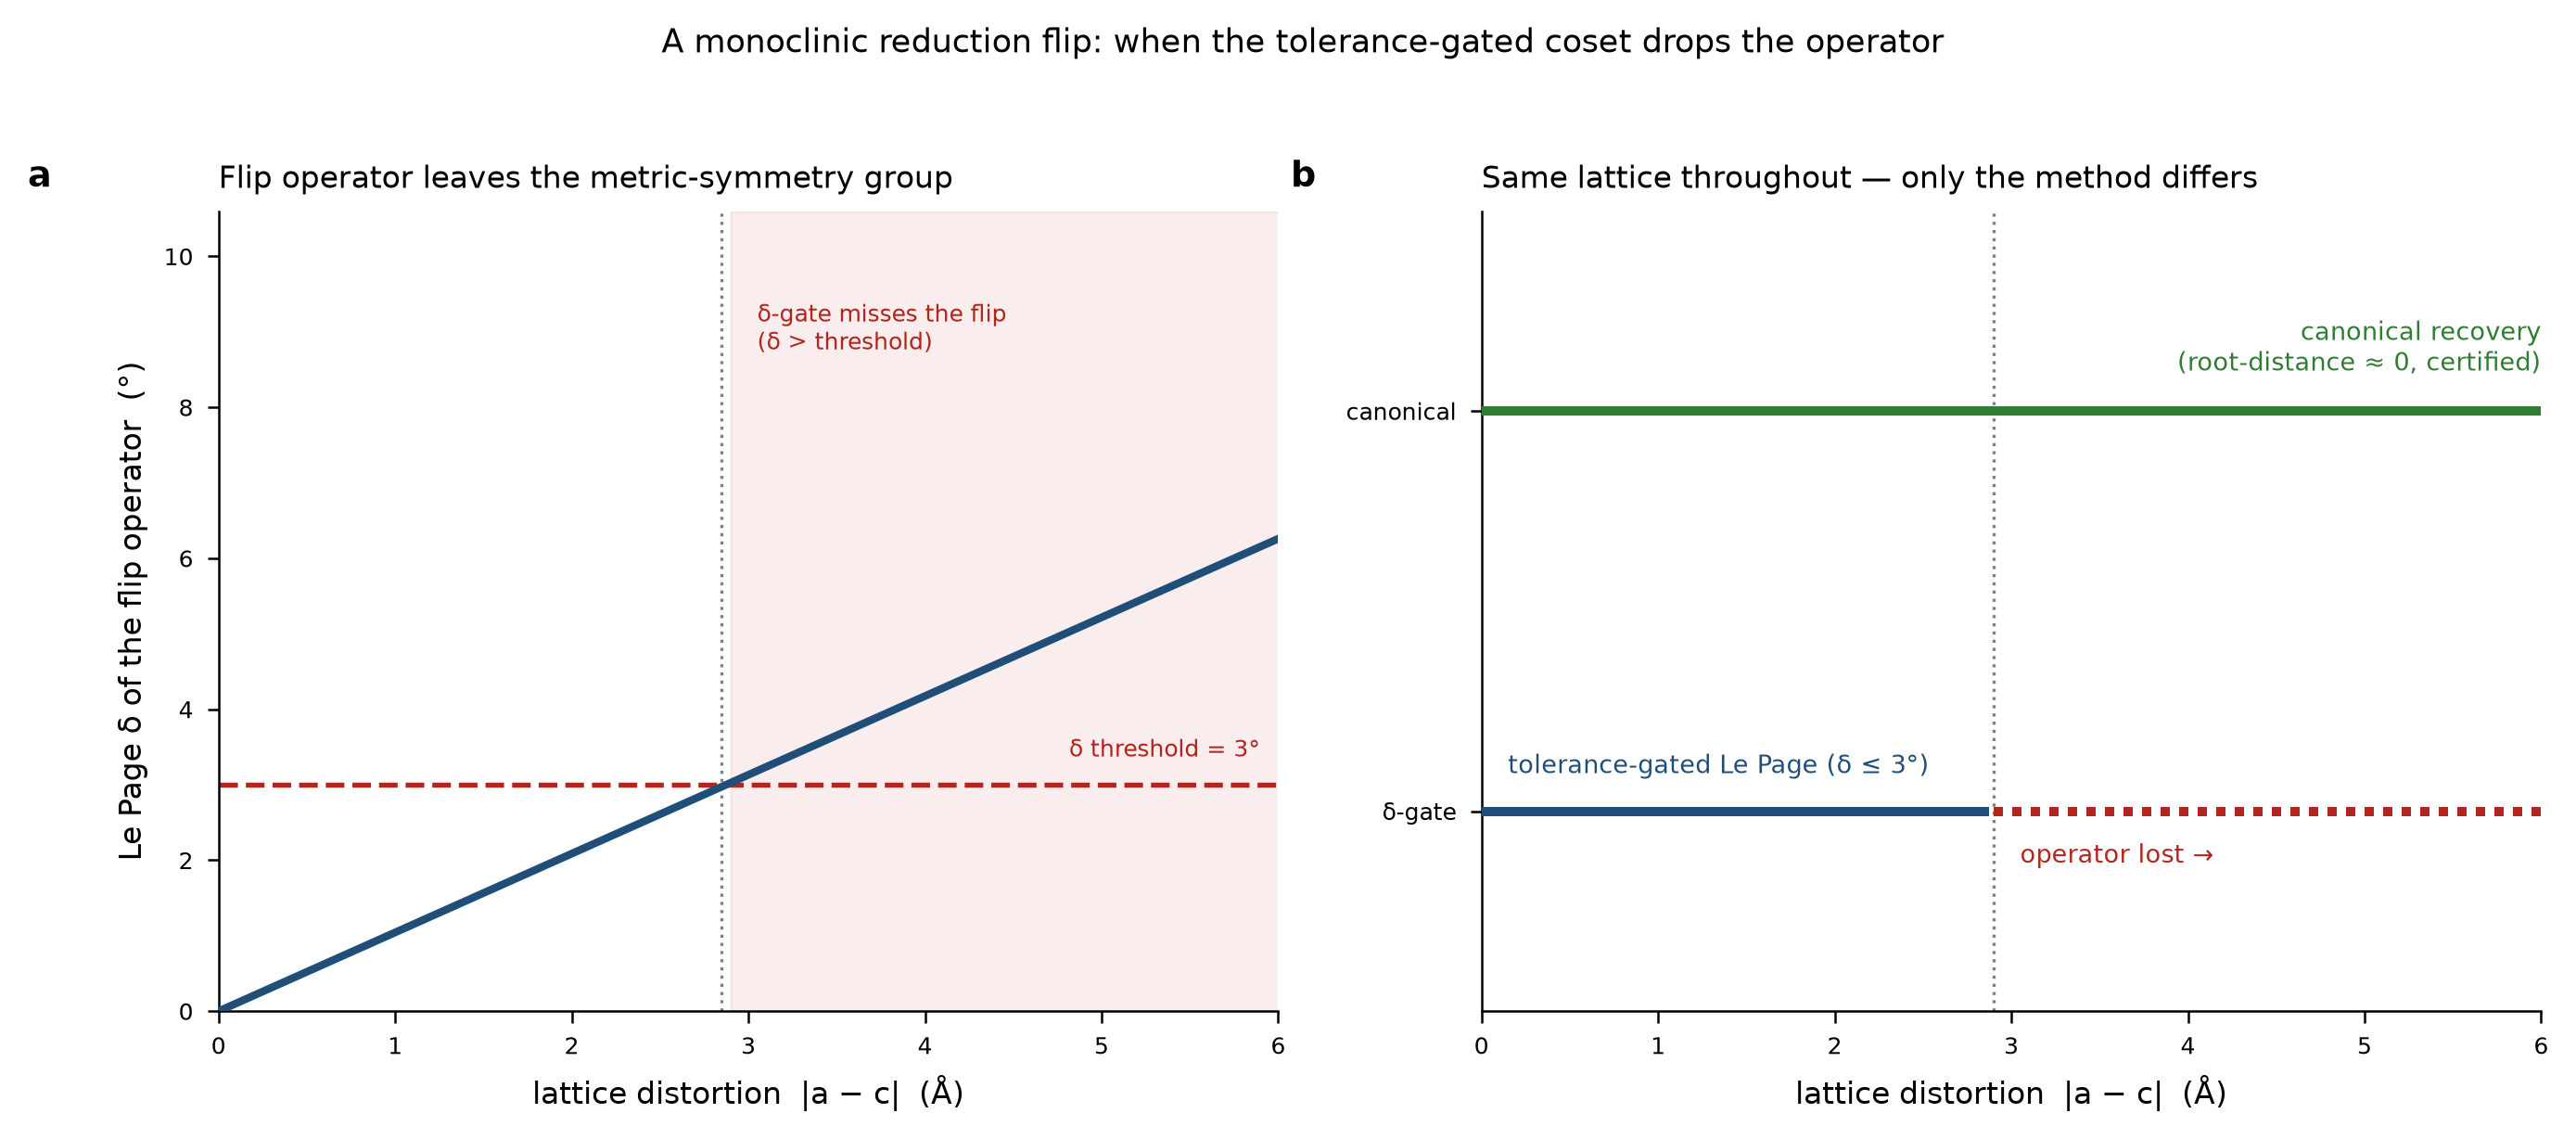
\includegraphics[width=\linewidth]{figure3.png}
\caption{The reduction-flip gate. \textbf{(a)} As the monoclinic distortion
$|a-c|$ opens, the Le Page $\delta$ of the flip operator grows linearly and
crosses the $\delta$ threshold ($3\degree$) at $|a-c|\approx\SI{2.85}{\angstrom}$;
beyond it the tolerance gate no longer admits the operator (shaded).
\textbf{(b)} The two settings are the same lattice at every distortion
(root distance $\approx0$), so the canonical-superbase recovery (green) returns
the exact flip operator throughout, whereas the tolerance-gated coset (blue)
drops it past the crossing (red).}
\label{fig:flip}
\end{figure}

\emph{Why this is structural, not incidental.} The flip-free operator recovery is
the condition that turns a continuous \emph{parameterisation} of lattices into a
\emph{traversable} manifold, and this is what the programme in the Discussion ---
lattices as a continuum, trajectories in place of independent refinements ---
actually requires. Two properties must hold together. The coordinate must be
continuous, so that neighbouring lattices receive neighbouring invariants; the
root invariant supplies this. And motion along the manifold must be well defined,
so that a state can be related to its neighbour by an exact operator and a
trajectory is a composable sequence of steps rather than an unlinked cloud of
points; the canonical-superbase recovery supplies this. The reduction flip is
precisely the obstruction to the second property, and it strikes where it matters
most: the degeneracies at which a tolerance gate drops the connecting operator are
the higher-symmetry loci --- the phase transitions, symmetry-breaking events and
trajectory junctions where the interesting physics lives. A continuum description
that fails at its own symmetry points is not a continuum description. The two
guarantees are in fact one fact seen twice: the invariant is flip-free as a
\emph{value} (it does not jump at a reduction boundary, because it lives on the
quotient rather than on a section), and the operator recovery is flip-free as a
\emph{map} (the connecting operator is returned exactly, because the two settings
have zero root distance) --- both because the boundary at which a section flips is
an ordinary interior point of the quotient. Continuity of the coordinate and
recoverability of the connecting operator are two faces of the same property, and
together they make the lattice continuum not merely parameterisable but connected
by exact operators through its symmetry loci. Concretely, this is what closes a
deformation trajectory that passes through a symmetry junction: the composed
path operator remains an exact integer unimodular matrix across the junction, so a
path that leaves a state, crosses a higher-symmetry point and returns is
holonomy-consistent rather than accumulating a silently dropped flip
(Section~\ref{sec:benchmarks}).

% ------------------------------------------------------------
\section{Results}

\subsection{An entire protein census on one metric (1361 archival cells)}

We retrieved every hen egg-white lysozyme entry in the PDB (UniProt P00698):
1372 entries, 1361 with a crystallographic cell. These span six space groups and
four crystal systems --- $P4_32_12$ tetragonal (1152 cells, 85\%),
$P2_12_12_1$ orthorhombic (100), $P2_1$ monoclinic (59), $P1$ triclinic (41),
and small hexagonal/trigonal minorities. Compared as raw six-tuples these would
scatter identical lattices into different points and merge unrelated ones;
compared as root invariants they collapse onto a single setting-invariant metric
(Fig.~\ref{fig:realdata}a) in which each crystal system occupies a distinct,
coherent region and the full $1361 \times 1361$ root-distance matrix is
meaningful across systems at once.

Within the dominant tetragonal form the 1113 native-volume cells
($a \approx b$, all angles fixed) are not a point but a continuous body spanning
a 26\% volume range. Because this subset is high-symmetry and single-setting it
is fully described by $(a, c)$; the invariant is not strictly required
\emph{here}, but it is what isolated this clean subset from the six-space-group
census in the first place. The second Laplacian eigenvector of the root-distance
graph --- the smoothest intrinsic coordinate on the manifold --- recovers the
cell-shrinkage axis at $|r| = 0.92$ (Fig.~\ref{fig:realdata}c). Parameterising by
this coordinate $t \in [0, 1]$ gives a smooth, monotone $a(t)$ rising
$76.8 \rightarrow 80.0\,\Ang$, while $c(t)$ is near-flat with a step from
$\approx 37.0$ to $\approx 38.0\,\Ang$ (Fig.~\ref{fig:realdata}b): the
deformation is anisotropic and staged --- the $a$-axis expands continuously
while $c$ shifts between two preferred hydration configurations --- consistent
with a dehydration series. The path is a curved arc through invariant space
(arc/chord $\approx 1.18$), the bend recording the staged repacking that a single
endpoint comparison discards. This is the manifold picture on real archival data:
a ``diverse'' census of 1361 independent determinations resolved into a handful
of crystal forms plus one continuous, physically interpretable deformation
coordinate.

\subsection{A complete serial XFEL indexing stream (12\,474 crystals)}

Merged depositions report one cell per structure. The per-pattern indexed-cell
distribution --- where reindexing ambiguity, cell scatter and misindexing
actually live --- is visible only in the primary indexing output. We parsed the
CrystFEL stream for a $\beta$-lactamase (BlaC) serial data set (CXIDB entry 83;
\SI{222}{\mega\byte} indexing stream) with a dependency-free reader added to the
package: 14\,445 diffraction patterns, 12\,474 indexed crystals (86\% rate),
space group $P6_3$, hexagonal ($\approx 41.8 \times 41.8 \times 233\,\Ang$).

The 12\,474 per-pattern cells form a cloud that the single merged deposition
reduces to one point (Fig.~\ref{fig:realdata}d). The long $c$-axis has a sharp
core (median $233.3\,\Ang$, median absolute deviation only $0.13\,\Ang$) with a
heavy tail to $245\,\Ang$; in the root-invariant manifold these cells form one
connected body with a smooth $c$-gradient (Fig.~\ref{fig:realdata}e), confirming
a genuine one-parameter spread rather than discrete misindexing classes.

Because the root invariant is orientation-blind by construction, colouring the
manifold by each crystal's orientation is a direct bias test: an unbiased data
set should show orientation scattered randomly across the manifold, and it
largely does. The residual weak coupling it exposes is physically real and
diagnostic (Fig.~\ref{fig:realdata}f): crystals struck with the beam nearly
parallel to $c^*$ determine the $233\,\Ang$ axis about $3\times$ more poorly
($c$-scatter $1.53\,\Ang$ for beam within $10\degree$ of $c^*$, versus
$\approx 0.5\,\Ang$ near the $ab$-plane), because reflections fixing the long
axis are poorly sampled when looking down it. The manifold's tail is therefore
enriched in an identifiable orientation class --- a concrete signal for
down-weighting those crystals in merging, and evidence that part of the apparent
$c$-axis spread is a sampling artifact, not lattice variation. Orientation itself
is uniformly distributed and handedness consistent, as expected for serial
crystallography; the $P6_3$ merohedral ambiguity resides in the reindexing coset,
which geometry surfaces and intensities resolve.

\subsection{Benchmarks and continuous trajectories}
\label{sec:benchmarks}

\paragraph{Database search.}
Because the root invariant is a fixed six-vector in Angstrom, exact
nearest-neighbour search uses a \texttt{scipy.spatial.cKDTree} on the
precomputed root components (a pure-Python metric NearTree [Andrews \& Bernstein,
2016] is retained only for non-Euclidean $G^6$/$S^6$ distances). Over 3000
perturbed cells the index builds in \SI{0.04}{\second}; 40/40 exact
nearest-neighbour queries recovered the planted cell at a median
\SI{0.02}{\milli\second}, and queries placed on opposite sides of a reduction
boundary returned the same reference lattice. On the full PDB holdings
(206\,214 cells) the same index builds in \SI{0.28}{\second} with median
\SI{0.04}{\milli\second} $k{=}10$ queries. The invariant performs the
high-volume filtering; equation~\eqref{eq:lift} is evaluated only for returned
neighbours. Volume-spanning searches first enumerate low-index
Hermite-normal-form sublattices, reduce and deduplicate them by root invariant,
and query each distinct lattice --- surfacing rather than hiding supercell
non-uniqueness (an orthorhombic $40/50/60\,\Ang$ lattice has seven distinct
index-two sublattices, all kept as separate candidates).

\paragraph{Serial reindexing.}
On 200 perturbed monoclinic frames including settings on both sides of a
reduction flip, a brute-force reference tested 6960 small unimodular matrices per
frame at \SI{23}{\milli\second} per frame; the root-first workflow established
identity, lifted each frame through its canonical superbase, and reduced the
admissible result to a cached two-operator reference coset tested at
\SI{0.07}{\milli\second} per frame --- a $\approx 330$-fold per-frame reduction
($\approx 180$-fold amortised). Geometry returns the exact admissible operators;
intensity correlation remains the tie-breaker when two coset representatives are
metrically equivalent [Brehm \& Diederichs, 2014; Gildea \& Winter, 2018].

\paragraph{Deformation trajectory.}
A synthetic 41-cell monoclinic series shrinking $c$ from 150 to $100\,\Ang$
($a = 120$, $b = 189.1\,\Ang$, $\beta = 91.2\degree$) passes through $a = c$ at
$t = 0.60$, where axis exchange becomes an exact lattice symmetry. The Fiedler
coordinate [Fiedler, 1973] of a four-neighbour root-distance graph recovered the
imposed coordinate at $|r| = 0.9913$; the accumulated adjacent path length was
$50.13\,\Ang$ versus a $35.88\,\Ang$ endpoint chord --- the difference recording
deformation a single comparison discards. The root graph supplies the order; the
canonical-superbase lift supplies local frames attached at the two endpoints and
the symmetry junction. No tolerance makes one exact integer operator map the two
deliberately different endpoints; the path is part of the answer.

\paragraph{Archival-scale similarity embedding.}
Volume-normalised root invariants $s = \mathrm{RI}/V^{1/3}$ place every PDB
cell in a common shape space. Embedding the full holdings (206\,214 cells) with
a metric-neighbourhood network into a two-dimensional latent plane yields a
continuous census in which crystal systems occupy coherent regions. To ask how
many independent shape degrees of freedom remain \emph{locally}, we tile the
latent plane with unit centres and, in each ball of radius $0.5$, compute a
mean-centred SVD of the six-vector $s$. The local dimensionality is the
entropy (Roy--Vetterli) effective rank
$\exp\bigl(-\sum_i p_i\ln p_i\bigr)$ with $p_i=\sigma_i/\sum_j\sigma_j$; empty
cells and balls with fewer than two points are scored zero
(Fig.~\ref{fig:localdim}). Of 570 grid cells, 322 are occupied; among those the
effective rank has median $4.12$ and spans roughly $1$--$5.1$. High-rank
patches mark fuller local variation of the similarity invariant; low-rank
filaments are locally near one-parameter families --- the same continuous
geometry the smaller lysozyme and XFEL manifolds already illustrated, now read
off the archive as a whole.

% --- Figure 1 ---
\begin{figure}[t]
\centering
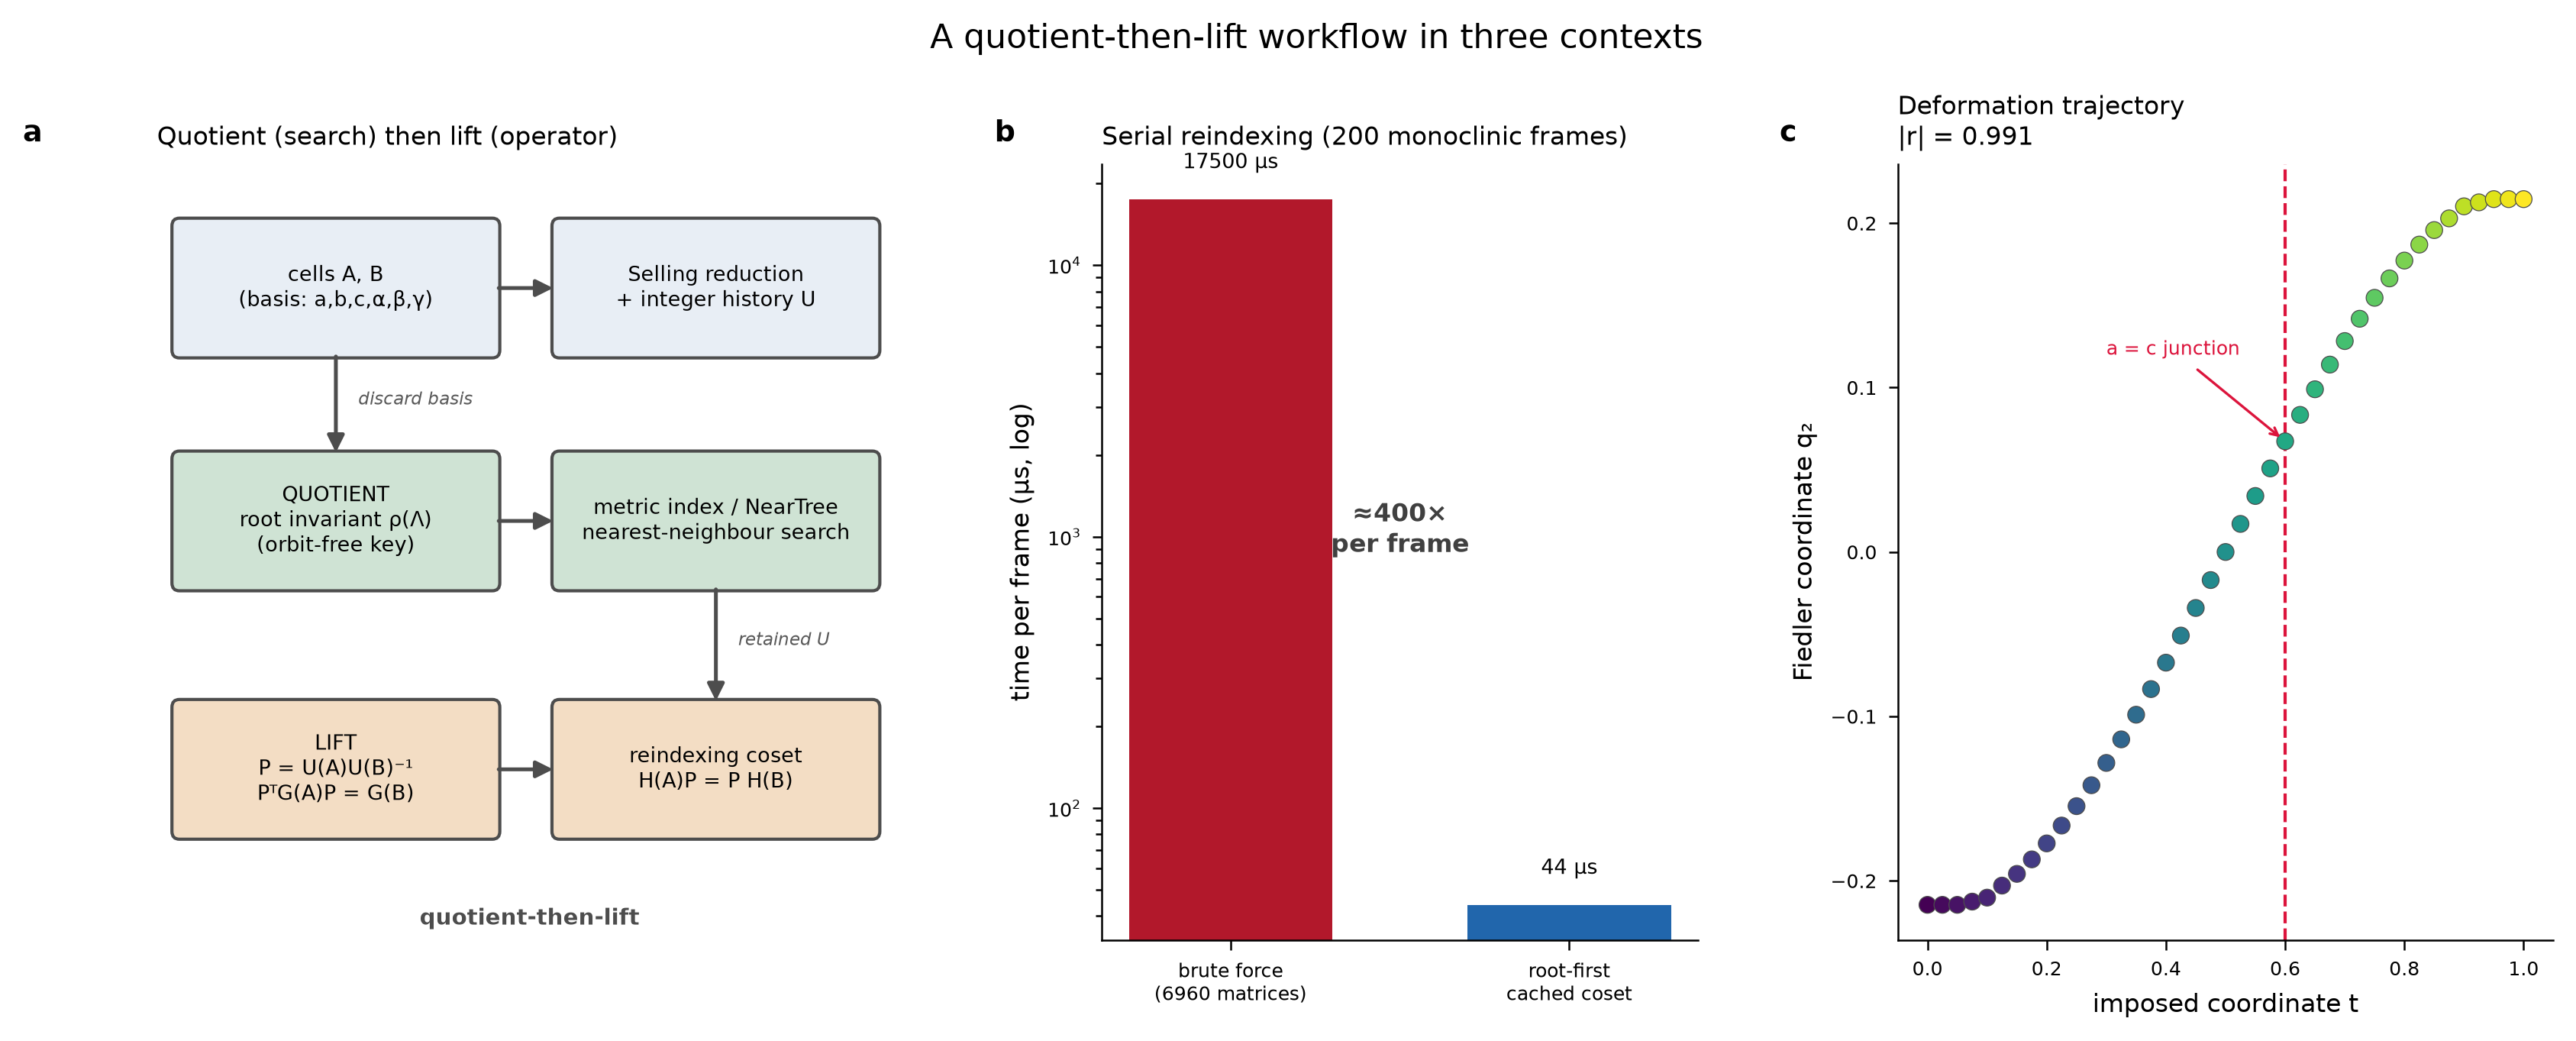
\includegraphics[width=\textwidth]{figure1.png}
\caption{The quotient-then-lift workflow. Root invariants supply a
basis-independent metric index; integer coordinates retained during
canonical-superbase construction lift selected neighbours back to explicit
operators by $\Pop = \Uop(A)\Uop(B)^{-1}$. (a) Two-dimensional projection of the
3000-cell nearest-neighbour index. (b) Serial benchmark: repeated 6960-matrix
search versus a cached two-operator reference coset. (c) Root-distance graph for
the 41-state shrinkage trajectory, with local operators attached at the endpoints
and the $a = c$ junction. Projection geometry in (a) and (c) is illustrative;
numerical annotations are from the six-dimensional calculations.}
\label{fig:workflow}
\end{figure}

% --- Figure 2 ---
\begin{figure*}[t]
\centering
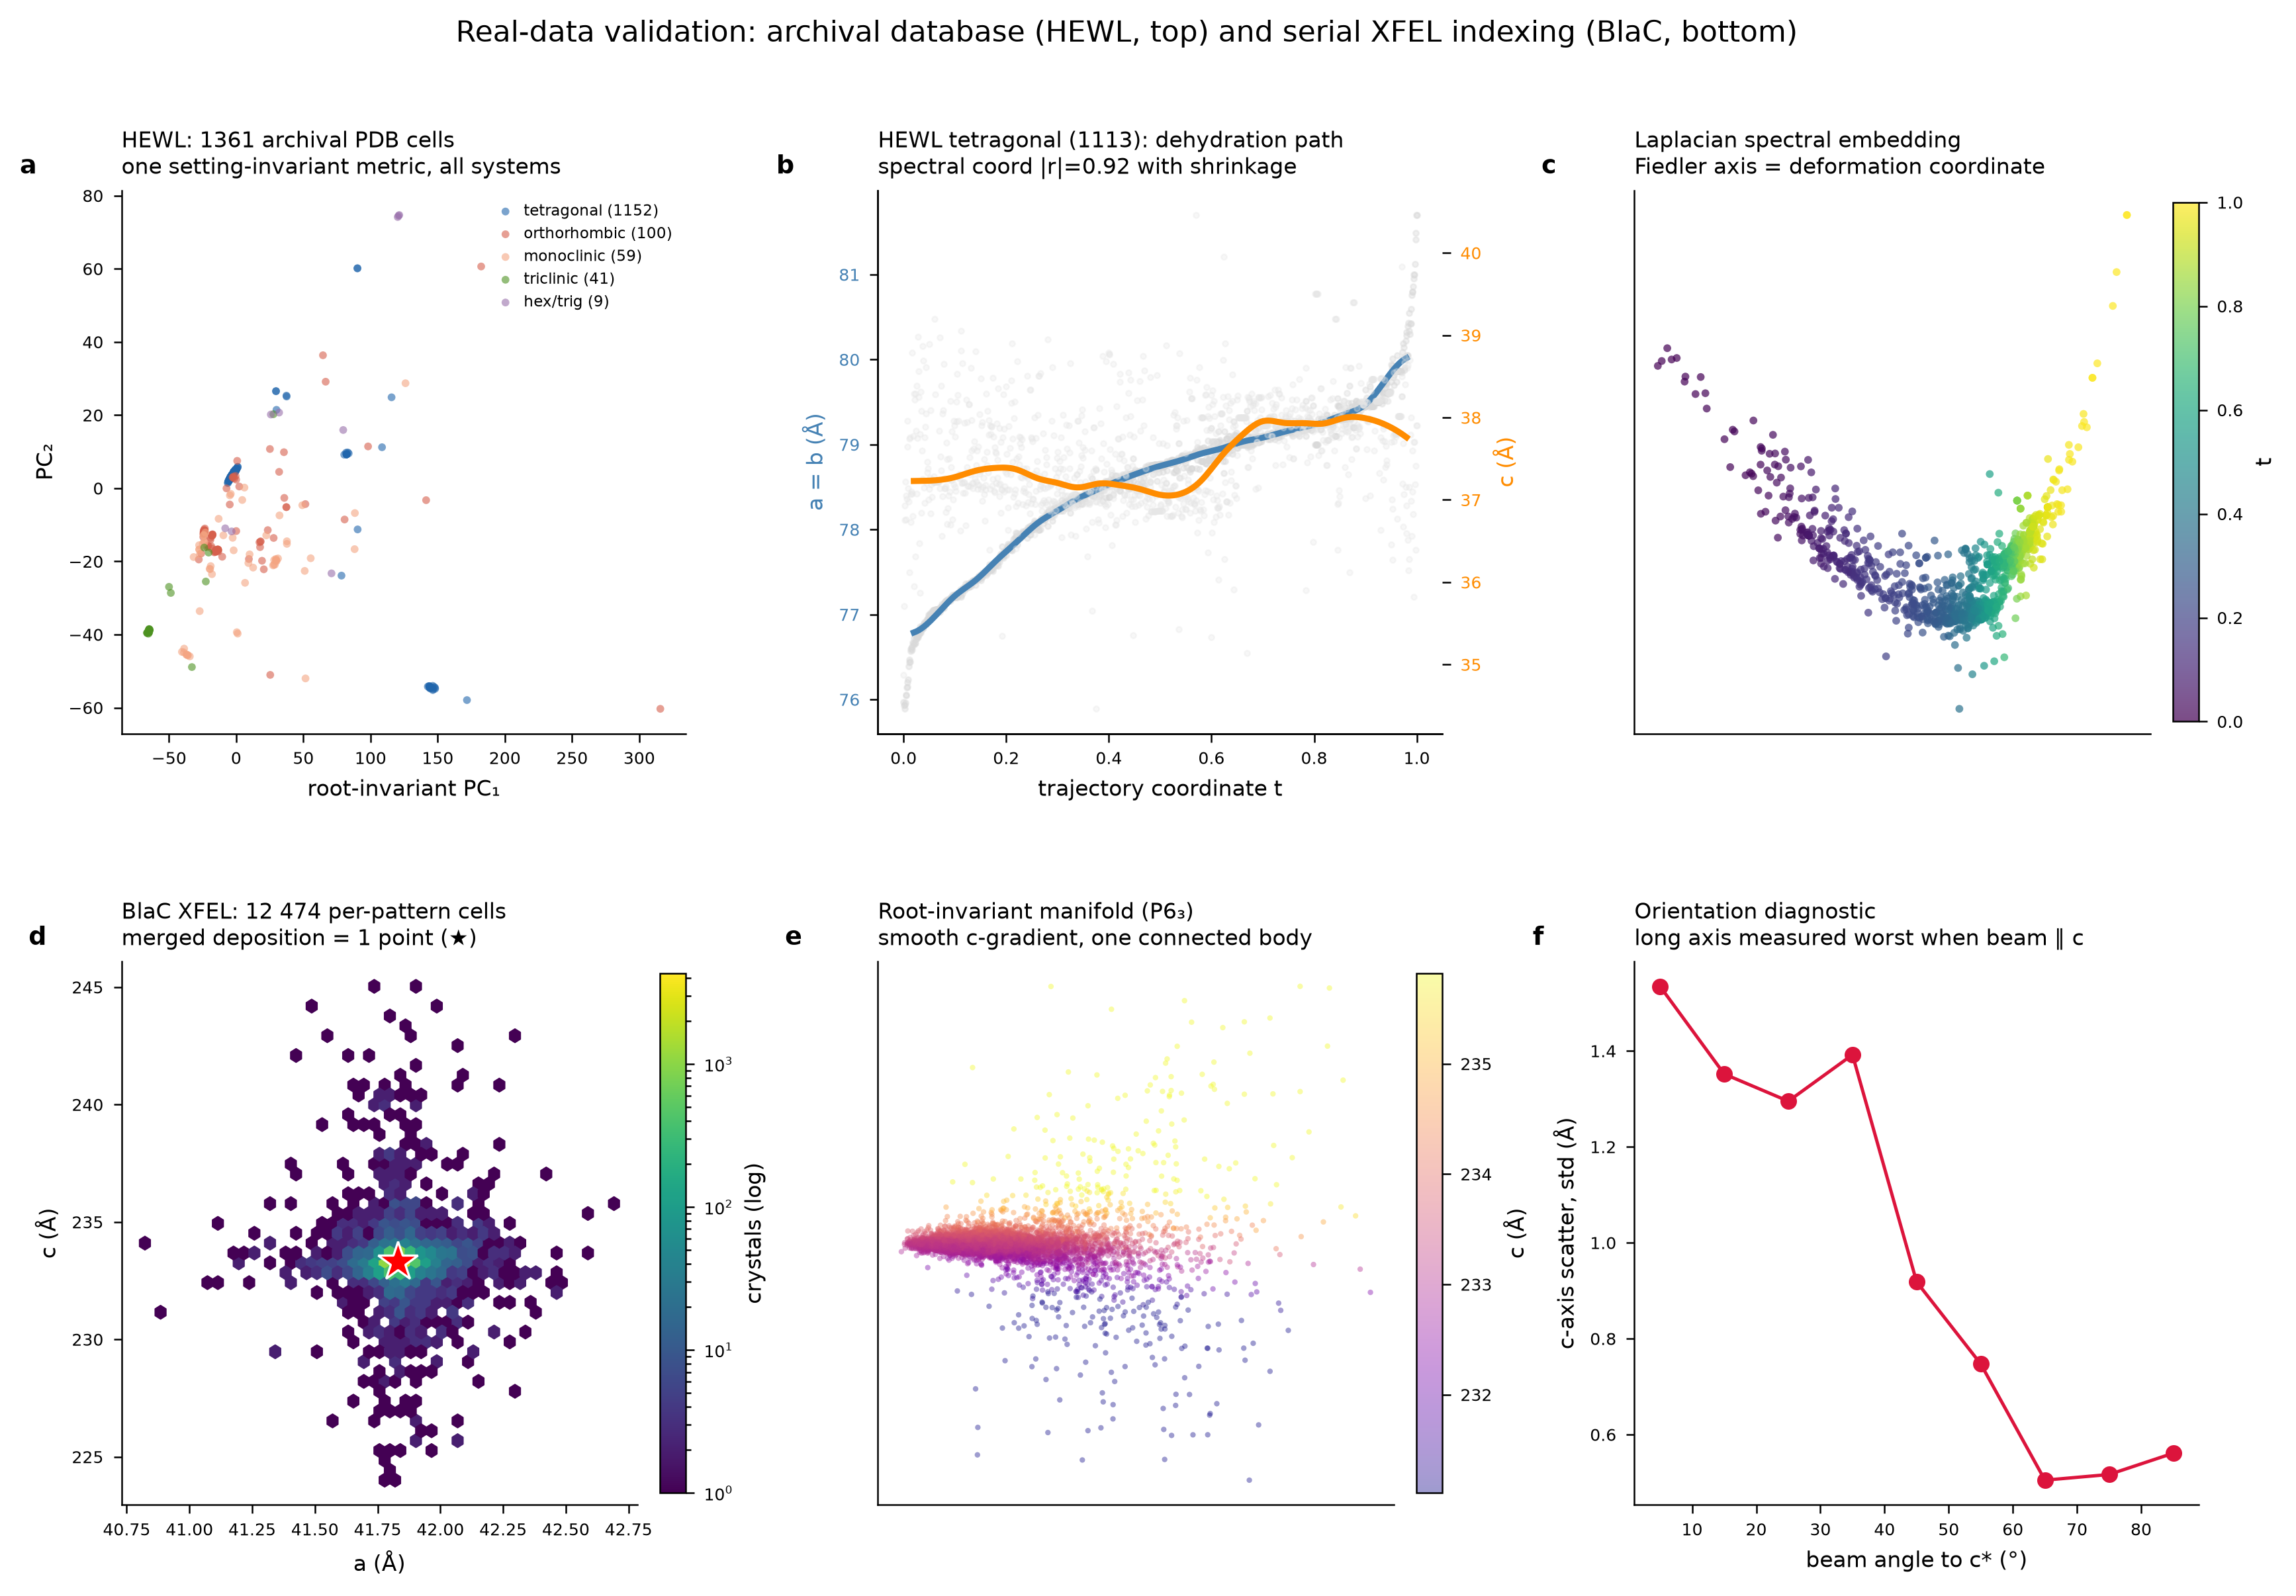
\includegraphics[width=\textwidth]{figure2.png}
\caption{Real-data validation. Top --- an archival database census (hen egg-white
lysozyme, 1361 PDB cells): (a) all six space groups and four crystal systems on
one setting-invariant root-invariant metric; (b) within the 1113-cell native
tetragonal form, $a(t)$ and $c(t)$ along the intrinsic deformation coordinate
show anisotropic, staged dehydration; (c) Laplacian spectral embedding whose
Fiedler axis recovers cell shrinkage ($|r| = 0.92$). Bottom --- a complete serial
XFEL indexing stream ($\beta$-lactamase, CXIDB 83, 12\,474 indexed crystals,
$P6_3$): (d) the per-pattern indexed-cell cloud that the merged deposition
collapses to one point ($\star$); (e) the root-invariant manifold coloured by
$c$, one connected body with a smooth gradient; (f) orientation diagnostic ---
the $233\,\Ang$ axis is measured worst (largest per-pattern $c$-scatter) when the
beam looks down $c^*$.}
\label{fig:realdata}
\end{figure*}

\begin{figure}[t]
\centering
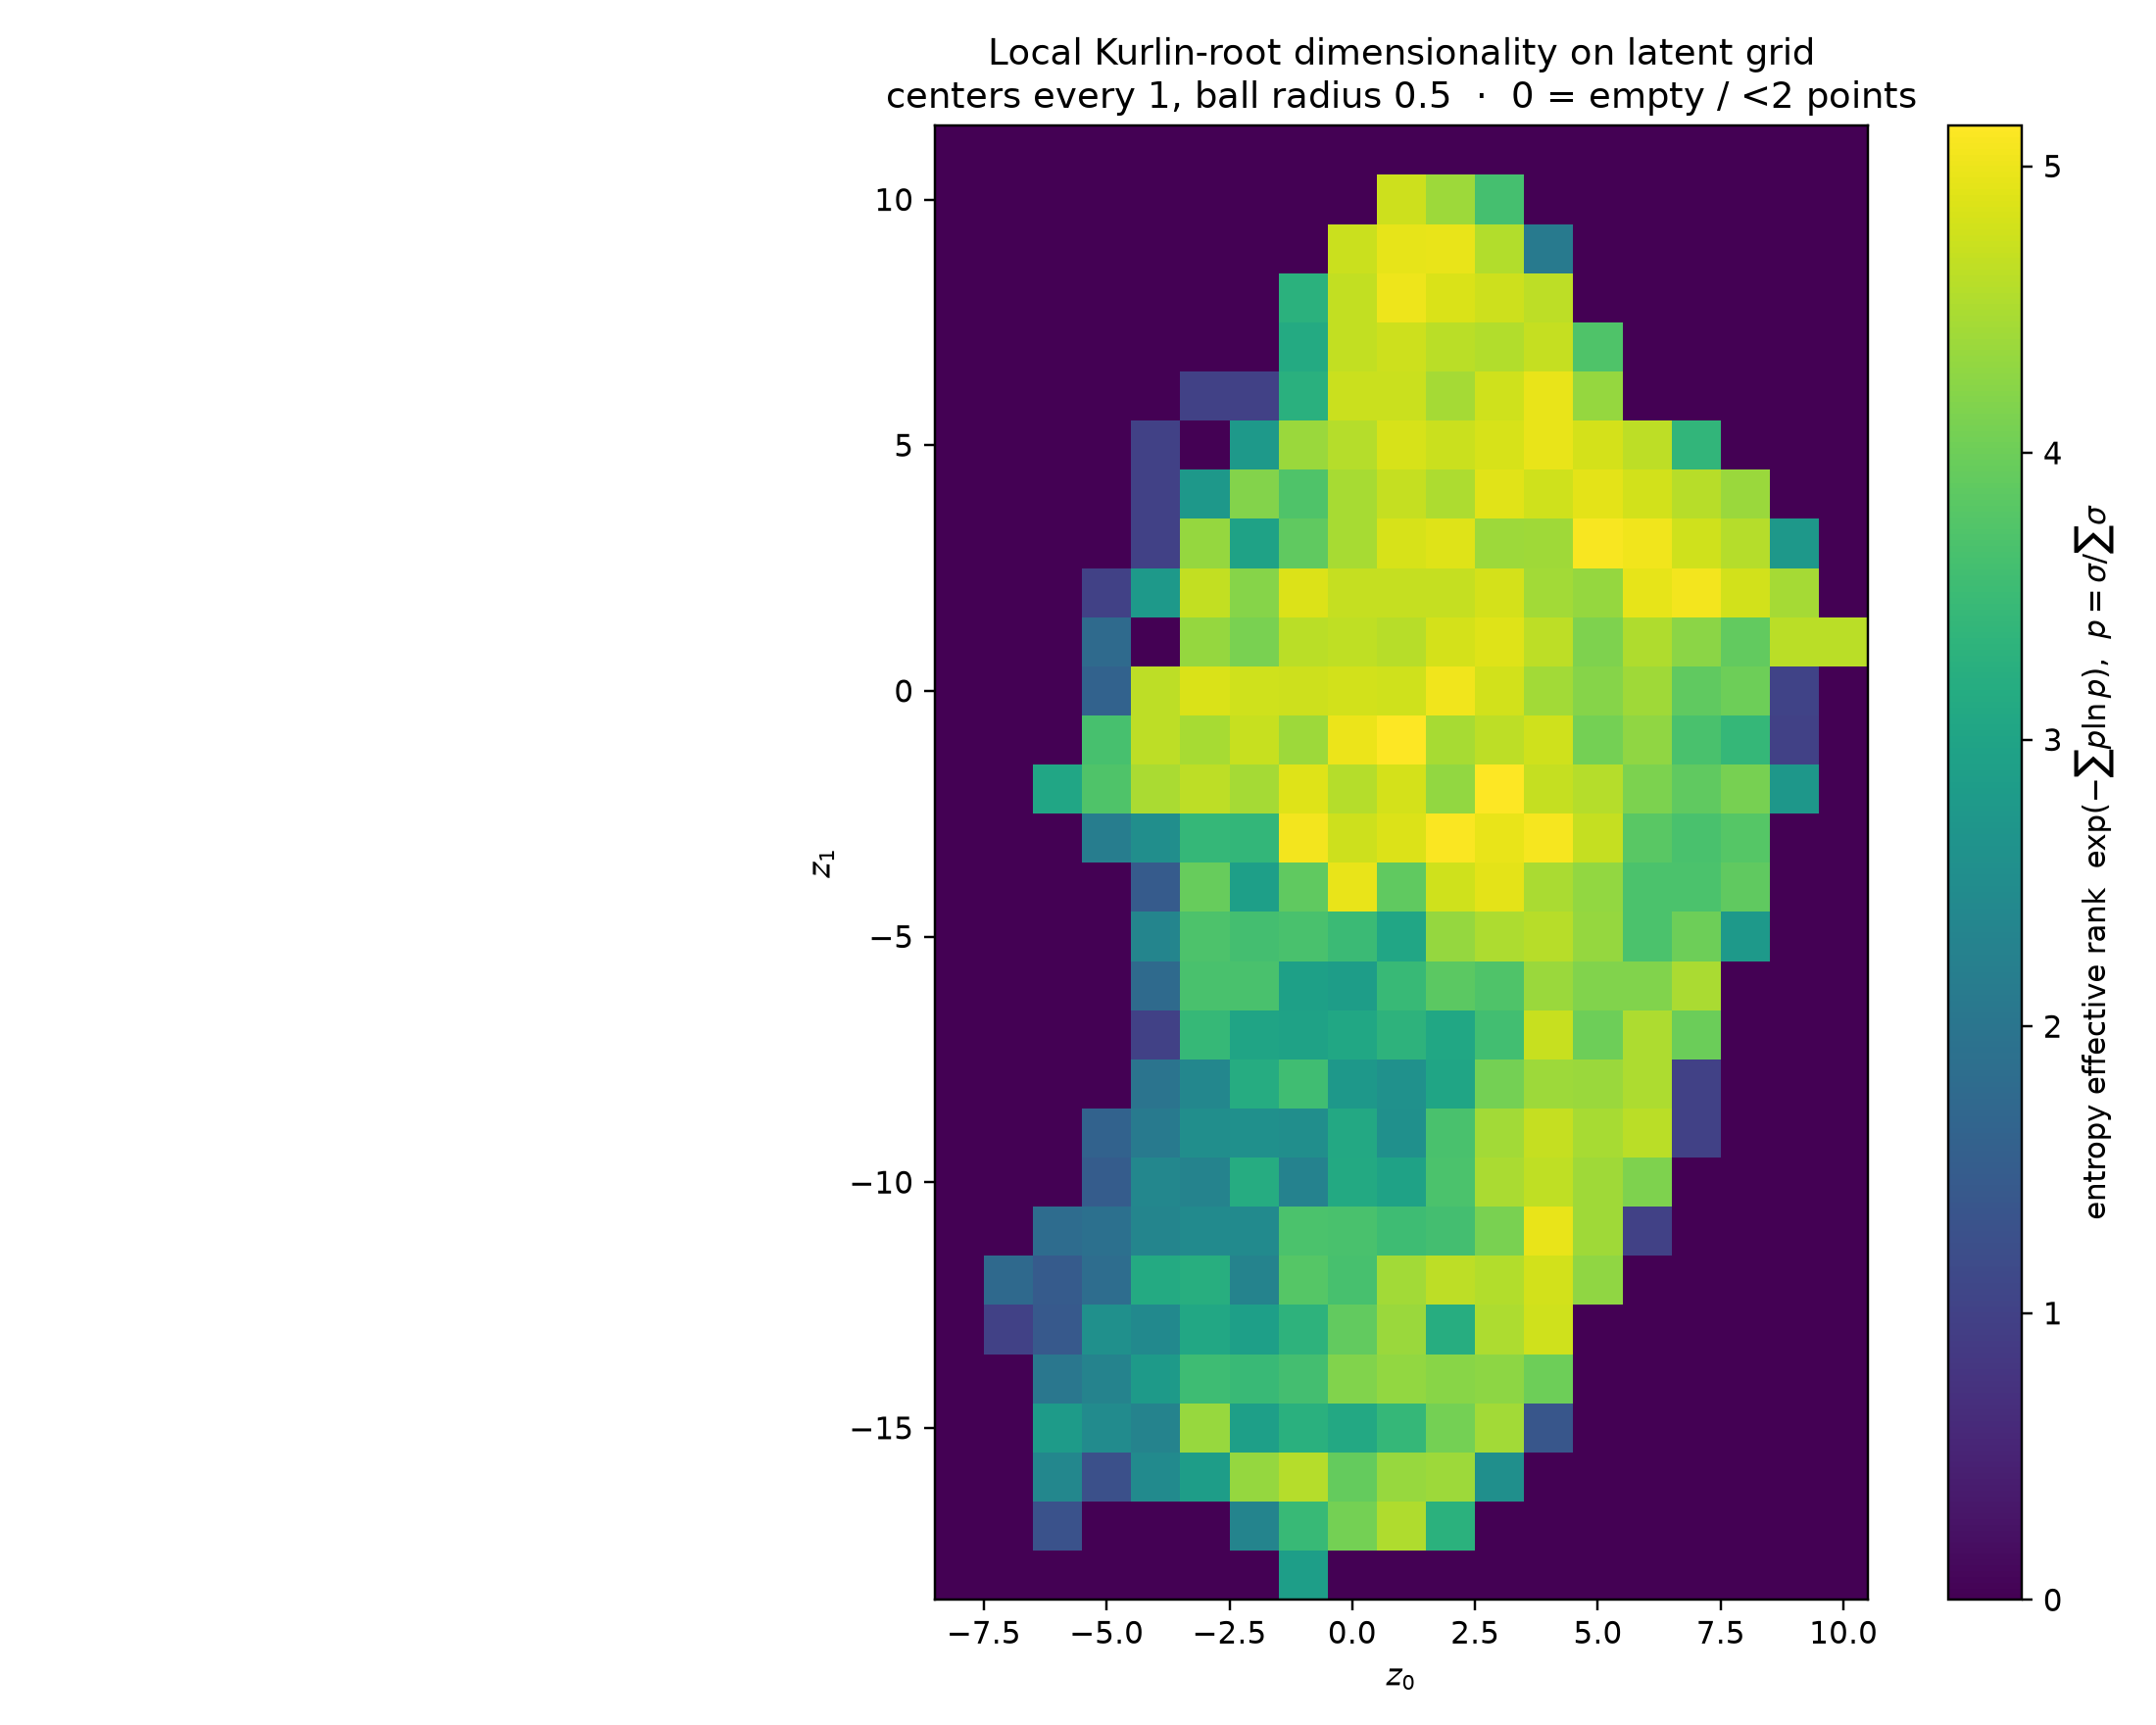
\includegraphics[width=\textwidth]{figure4.png}
\caption{Local dimensionality of the PDB similarity embedding. Unit grid on
the two-dimensional latent plane of 206\,214 volume-normalised root invariants;
colour is the entropy effective rank of a mean-centred SVD of $s=\mathrm{RI}/V^{1/3}$
inside a ball of radius $0.5$ (zero where empty or $n{<}2$). Occupied cells
span effective ranks $\approx 1$--$5.1$ (median $4.12$).}
\label{fig:localdim}
\end{figure}

% ------------------------------------------------------------
\section{Discussion}

The useful distinction is between a quotient and a lift. $G^6$ and $S^6$ provide
physically meaningful coordinates, but a lattice distance in either must account
for equivalent presentations and glued boundaries. The root invariant performs
that quotient once, giving a continuous key suitable for large-scale search;
retaining the integer reduction history then lifts a selected match back to the
basis-level operator that crystallographic processing needs. This prevents three
category errors: treating alternative bases as different database entries, using
a lattice-identity test as though it already specified the reflection reindexing,
and forcing distant states of a deformation into one pairwise integer map.

The real-data cases show the construction is not merely a benchmark convenience.
A whole-protein PDB census reduces to one cross-system metric on which a genuine
deformation trajectory is legible; a complete serial XFEL stream exposes a
per-pattern cell distribution that every merged deposition hides, and the
orientation-blindness of the invariant becomes an experimental diagnostic rather
than a limitation. The archival similarity embedding and its local entropy-rank map
(Fig.~\ref{fig:localdim}) extend that picture from single-protein and single-
experiment manifolds to the full PDB shape census. The remaining work is
validation depth, not scope: database timing on archival-scale, multi-protein
holdings is now included (206\,214 PDB cells, Section~\ref{sec:benchmarks});
serial validation against experimental intensities and production reindexing
decisions; and trajectory transport on measured thermal, time-resolved or
operando series with uncertainty propagation and cycle-consistency diagnostics. The central algorithmic claim is
narrow and, we believe, now well supported: similarity need not be solved by an
orbit search, and recovering the operator need not reopen the unrestricted search
the invariant eliminated. None of the underlying mathematics is new to this
paper; the completeness and continuity that make all of this work are Kurlin's
(2022). What we add is the crossing --- expressing that result in crystallographic
terms, connecting it to the reduction-flip and reindexing problems the field
actually faces, and delivering it as software validated at data scale --- so that
a complete invariant already available in the lattice-geometry literature becomes
usable where diffraction data are processed.

% ------------------------------------------------------------
\section*{Data and code availability}

The implementation (a dependency-free Python package with a zero-dependency
runtime and oracle-validated test suite), the CrystFEL stream parser, benchmark
inputs, and the scripts generating Figs~1 and~2 will be deposited in a versioned
public repository before submission. The lysozyme cells derive from public PDB
entries (UniProt P00698). The serial data are a $\beta$-lactamase XFEL data set
deposited as CXIDB entry 83. [Authors to confirm the CXIDB accession and add its
primary citation.] [Insert repository URL and archival DOI.]

\section*{Acknowledgements}

[Insert funding and acknowledgements.] \emph{AI-tool disclosure} [confirm before
submission]: Generative AI tools were used for exploratory coding and language
editing. All algorithms, numerical results, references and scientific claims were
independently checked and approved by the authors.

% ------------------------------------------------------------
\begin{thebibliography}{99}
\small

\bibitem{ab1988} Andrews, L. C. \& Bernstein, H. J. (1988).
\textit{Acta Cryst.} A\textbf{44}, 1009--1018.

\bibitem{ab2014} Andrews, L. C. \& Bernstein, H. J. (2014).
\textit{J. Appl. Cryst.} \textbf{47}, 346--359.

\bibitem{ab2016} Andrews, L. C. \& Bernstein, H. J. (2016).
\textit{J. Appl. Cryst.} \textbf{49}, 756--761.

\bibitem{abs2019} Andrews, L. C., Bernstein, H. J. \& Sauter, N. K. (2019).
\textit{Acta Cryst.} A\textbf{75}, 593--599.

\bibitem{ab2023} Andrews, L. C. \& Bernstein, H. J. (2023).
\textit{Acta Cryst.} A\textbf{79}, 485--498.

\bibitem{bd2014} Brehm, W. \& Diederichs, K. (2014).
\textit{Acta Cryst.} D\textbf{70}, 101--109.

\bibitem{bck2021} Bright, M., Cooper, A. I. \& Kurlin, V. (2021).
A complete and continuous map of the Lattice Isometry Space for all
3-dimensional lattices. \texttt{arXiv:2109.11538}.

\bibitem{fiedler1973} Fiedler, M. (1973).
\textit{Czechoslovak Math. J.} \textbf{23}, 298--305.

\bibitem{gw2018} Gildea, R. J. \& Winter, G. (2018).
\textit{Acta Cryst.} D\textbf{74}, 405--410.

\bibitem{kurlin2022} Kurlin, V. (2022).
A complete isometry classification of 3-dimensional lattices.
\texttt{arXiv:2201.10543}.

\end{thebibliography}

\end{document}
